\documentclass[12pt,a4paper]{report}

% ==============================================================================
% Packages & Configuration
% ==============================================================================
\usepackage[utf8]{inputenc}
\usepackage[T1]{fontenc}
\usepackage{mathptmx} % Times New Roman font for academic rigor
\usepackage[a4paper,top=1in,bottom=1in,left=1.2in,right=1in]{geometry}
\usepackage{setspace}
\onehalfspacing

\usepackage{graphicx}
\usepackage{xcolor}
\usepackage{amsmath,amssymb}
\usepackage{booktabs}
\usepackage{tabularx}
\usepackage{multirow}
\usepackage{array}
\usepackage{fancyhdr}
\usepackage{titlesec}
\usepackage{caption}
\usepackage{subcaption}
\usepackage{microtype}
\usepackage{cite}
\usepackage{tcolorbox}
\tcbuselibrary{skins,breakable}

% Hyperref configuration
\usepackage[colorlinks=true,
            linkcolor=mahenavy,
            citecolor=manipalrust,
            urlcolor=manipalrust,
            bookmarks=true,
            bookmarksnumbered=true]{hyperref}

% ==============================================================================
% Color Definitions (Derived from MAHE Identity & image2.png)
% ==============================================================================
\definecolor{manipalrust}{RGB}{196, 74, 30}     % Signature Manipal Rust/Burnt Orange (#C45A2C)
\definecolor{mahenavy}{RGB}{24, 43, 73}         % Formal Academic Navy
\definecolor{lightrust}{RGB}{253, 247, 243}      % Light accent tint
\definecolor{codebg}{RGB}{248, 249, 250}         % Subtle background for code/boxes
\definecolor{darkgray}{RGB}{60, 60, 60}

% ==============================================================================
% Section Heading Styling
% ==============================================================================
\titleformat{\chapter}[display]
  {\normalfont\huge\bfseries\color{manipalrust}}
  {\filleft\Huge\color{gray!60}Chapter \thechapter}
  {1ex}
  {\titlerule[1.5pt]\vspace{1.5ex}\filright}
  [\vspace{1.5ex}\titlerule]

\titleformat{\section}
  {\normalfont\Large\bfseries\color{mahenavy}}
  {\thesection}{1em}{}

\titleformat{\subsection}
  {\normalfont\large\bfseries\color{manipalrust}}
  {\thesubsection}{1em}{}

\titleformat{\subsubsection}
  {\normalfont\normalsize\bfseries\color{darkgray}}
  {\thesubsubsection}{1em}{}

% Captions
\captionsetup{font=small,labelfont={bf,color=manipalrust},labelsep=period}

% Header and Footer Styling
\pagestyle{fancy}
\fancyhf{}
\fancyhead[L]{\small\color{darkgray}\nouppercase{\leftmark}}
\fancyhead[R]{\small\color{manipalrust}\textbf{Multi-Agent LLM Systems}}
\fancyfoot[C]{\thepage}
\renewcommand{\headrulewidth}{0.5pt}
\renewcommand{\footrulewidth}{0pt}

% Callout Box Environment
\newtcolorbox{infobox}[1]{
  colback=lightrust,
  colframe=manipalrust,
  fonttitle=\bfseries\color{white},
  coltitle=white,
  title=#1,
  arc=2mm,
  boxrule=1pt,
  left=10pt,
  right=10pt,
  top=8pt,
  bottom=8pt
}

\begin{document}

% ==============================================================================
% COVER / TITLE PAGE (Strictly following image.png format + image2.png colors/logo)
% ==============================================================================
\begin{titlepage}
\centering
\thispagestyle{empty}

% Top Logo from image2.png
\includegraphics[width=0.72\textwidth]{figures/mahe_logo_clean.png}

\vspace{0.8cm}

{\fontsize{15}{18}\selectfont \textbf{Manipal School of Information Sciences}\par}

\vspace{1.0cm}

{\fontsize{13}{16}\selectfont A Seminar Report on\par}

\vspace{0.9cm}

% Seminar Title styled in image2.png primary color (Manipal Rust)
{\fontsize{18}{23}\selectfont \bfseries \color{manipalrust}
Multi-Agent LLM Systems: Workflow, Infrastructure, and Applications\par}

\vspace{1.2cm}

{\fontsize{11}{14}\selectfont Submitted in partial fulfillment of the requirements for the award of\par}

\vspace{0.3cm}

{\fontsize{13}{16}\selectfont \textbf{Master of Engineering (Computer Science and Engineering)}\par}

\vspace{1.2cm}

{\fontsize{11}{14}\selectfont Submitted by\par}

\vspace{0.3cm}

{\fontsize{14}{17}\selectfont \textbf{Varun B Karmikanda}\par}
\vspace{0.15cm}
{\fontsize{12}{15}\selectfont 261100610029\par}

\vspace{1.2cm}

{\fontsize{11}{14}\selectfont Under the guidance of\par}

\vspace{0.35cm}

{\fontsize{12}{15}\selectfont \textbf{Dr. Sathyendranath Malli} \quad \& \quad \textbf{Mr. Balaji B}\par}
\vspace{0.15cm}
{\fontsize{10}{13}\selectfont Associate Professor \hspace{2.8cm} Assistant Professor - Selection Grade\par}
\vspace{0.1cm}
{\fontsize{10}{13}\selectfont Manipal School of Information Sciences \hspace{0.5cm} Manipal School of Information Sciences\par}
\vspace{0.1cm}
{\fontsize{10}{13}\selectfont MAHE, Manipal \hspace{4.2cm} MAHE, Manipal\par}

\vfill

% Bottom Logo and Institutional Info from image2.png & image1

\includegraphics[width=0.55\textwidth]{figures/msis_logo.png}

\vspace{0.3cm}

{\fontsize{11}{14}\selectfont \textbf{Manipal School of Information Sciences}\par}
{\fontsize{10}{13}\selectfont \textbf{MAHE, Manipal}\par}
\vspace{0.15cm}
{\fontsize{10}{13}\selectfont \textbf{Academic Year 2026--27}\par}

\end{titlepage}

% ==============================================================================
% FRONT MATTER
% ==============================================================================
\pagenumbering{roman}
\setcounter{page}{2}

% ------------------------------------------------------------------------------
% Certificate
% ------------------------------------------------------------------------------
\newpage
\chapter*{Certificate}
\addcontentsline{toc}{chapter}{Certificate}

\noindent This is to certify that the Technical Seminar report entitled \textbf{``Multi-Agent LLM Systems: Workflow, Infrastructure, and Applications''} submitted by \textbf{Varun B Karmikanda} (Reg. No.: \textbf{261100610029}) in partial fulfillment of the requirements for the award of the degree of \textbf{Master of Engineering in Computer Science and Engineering} from \textbf{Manipal School of Information Sciences, Manipal Academy of Higher Education (MAHE), Manipal}, is a bonafide record of work carried out by him under our supervision and guidance during the academic year 2026--27.

\vspace{2.5cm}

\noindent
\begin{tabular*}{\textwidth}{@{\extracolsep{\fill}}cc}
\textbf{Dr. Sathyendranath Malli} & \textbf{Mr. Balaji B} \\
Guide, Associate Professor & Guide, Assistant Professor - Selection Grade \\
Manipal School of Information Sciences & Manipal School of Information Sciences \\
MAHE, Manipal & MAHE, Manipal \\
\end{tabular*}

\vspace{2.5cm}

\noindent
\begin{center}
\textbf{Director / Head of Department} \\
Manipal School of Information Sciences \\
Manipal Academy of Higher Education, Manipal
\end{center}

% ------------------------------------------------------------------------------
% Declaration
% ------------------------------------------------------------------------------
\newpage
\chapter*{Declaration}
\addcontentsline{toc}{chapter}{Declaration}

\noindent I hereby declare that the seminar report titled \textbf{``Multi-Agent LLM Systems: Workflow, Infrastructure, and Applications''} is an authentic presentation of my own academic seminar work carried out under the supervision of \textbf{Dr. Sathyendranath Malli} and \textbf{Mr. Balaji B}, Manipal School of Information Sciences, MAHE, Manipal.

\vspace{0.5cm}
\noindent I further declare that the content of this seminar report has not been submitted previously for the award of any degree, diploma, or fellowship in this or any other university or institute of learning. All literature, diagrams, survey data, and foundational references cited in this work have been duly acknowledged and referenced.

\vspace{2.0cm}

\noindent
\begin{tabular*}{\textwidth}{@{\extracolsep{\fill}}lr}
\textbf{Date:} 12/10/2026 & \textbf{Varun B Karmikanda} \\
\textbf{Place:} Manipal & Reg. No.: 261100610029 \\
& M.E. (Computer Science and Engineering) \\
\end{tabular*}

% ------------------------------------------------------------------------------
% Abstract
% ------------------------------------------------------------------------------
\newpage
\chapter*{Abstract}
\addcontentsline{toc}{chapter}{Abstract}

Large Language Models (LLMs) have achieved remarkable success across diverse natural language processing and synthetic reasoning tasks. However, when deployed in isolation as single, monolithic systems, LLMs exhibit fundamental limitations, including vulnerability to hallucinations, knowledge obsolescence, brittle multi-step reasoning, context length exhaustion, and an inherent inability to self-correct without external grounding. To overcome these constraints, the paradigm of \textbf{LLM-based Multi-Agent Systems (MAS)} has emerged as a transformative frontier in artificial intelligence. 

By decomposing complex goals across teams of specialized, communicative agents equipped with distinct personas, private memory, reasoning modules, and environmental tools, multi-agent frameworks facilitate collaborative problem-solving, iterative cross-checking, and dynamic world simulations. This seminar report provides an in-depth, structured review of LLM-based multi-agent systems, synthesized from authoritative literature including Li et al. (2024) and Guo et al. (2024). We analyze the transition from single-agent cognitive architectures to multi-agent teams, detailing the universal five-module workflow framework: \textit{Agent Profiling}, \textit{Perception}, \textit{Self-Action} (encompassing memory hierarchies, knowledge grounding, reasoning, and tool use), \textit{Mutual Interaction} (communication delivery, topological structures, and cooperative/adversarial scenes), and \textit{Evolution}. 

Furthermore, to bridge theoretical paradigms with empirical engineering, we present a concrete case study: an end-to-end \textbf{Autonomous Multi-Agent Research Assistant} implemented using LangChain and Groq API. The system orchestrates specialized Search, Reader, Writer, and Critic agents to autonomously discover, scrape, synthesize, and rigorously critique research reports. Finally, we survey real-world application domains across software engineering, scientific synthesis, and societal simulation, evaluate prevailing challenges including hallucination propagation, coordination overhead, and safety alignment, and discuss emerging frontiers including Agent-as-a-Service (AaaS) and the Model Context Protocol (MCP).

\vspace{0.8cm}
\noindent \textbf{Keywords:} Large Language Models, Multi-Agent Systems, Autonomous Agents, Agent Workflows, Cognitive Architectures, LangChain, Tool Use, Collective Intelligence.

% ------------------------------------------------------------------------------
% Acknowledgements
% ------------------------------------------------------------------------------
\newpage
\chapter*{Acknowledgements}
\addcontentsline{toc}{chapter}{Acknowledgements}

I would like to express my profound gratitude to my seminar guides, \textbf{Dr. Sathyendranath Malli}, Associate Professor, and \textbf{Mr. Balaji B}, Assistant Professor - Selection Grade, Manipal School of Information Sciences, MAHE, Manipal, for their invaluable guidance, encouragement, and insightful feedback throughout the preparation of this technical seminar report.

I extend my heartfelt appreciation to the faculty members and staff of the \textbf{Manipal School of Information Sciences (MSIS), Manipal Academy of Higher Education (MAHE)}, for providing the state-of-the-art computational infrastructure, academic resources, and conducive research atmosphere that enabled the completion of this study.

Lastly, I express my sincere thanks to my family, peers, and fellow researchers whose unwavering moral support, constructive critiques, and stimulating discussions have been instrumental throughout this endeavor.

\vspace{1.5cm}
\noindent \textbf{Varun B Karmikanda}

% ------------------------------------------------------------------------------
% Lists: TOC, LOF, LOT
% ------------------------------------------------------------------------------
\newpage
\tableofcontents

\newpage
\listoffigures

\newpage
\listoftables

% ==============================================================================
% MAIN CONTENT
% ==============================================================================
\newpage
\pagenumbering{arabic}
\setcounter{page}{1}

% ==============================================================================
% CHAPTER 1: INTRODUCTION
% ==============================================================================
\chapter{Introduction}
\label{chap:introduction}

\section{Background and Motivation}
Over the past several years, the rapid advancement of Large Language Models (LLMs)---such as GPT-4, Claude, Gemini, and open-weight models including LLaMA-3---has fundamentally altered the artificial intelligence landscape. Pre-trained on multi-terabyte textual corpora through autoregressive next-token prediction, modern LLMs possess extraordinary linguistic competence, zero-shot generalization, and emergent reasoning abilities \cite{wei2022chain}. 

Despite these impressive milestones, a standalone, monolithic LLM remains essentially a statistical text completion engine. In its bare form, an LLM operates on a synchronous \textit{request-to-response} loop: given an input prompt and static context window, the model produces a single output response through forward-pass inference, as illustrated in Figure~\ref{fig:llm_req_resp}. While sufficient for conversational question-answering and single-turn summarization, this static architecture cannot autonomously pursue long-horizon objectives, maintain state across days or weeks, or interactively manipulate external software environments.

\begin{figure}[htbp]
    \centering
    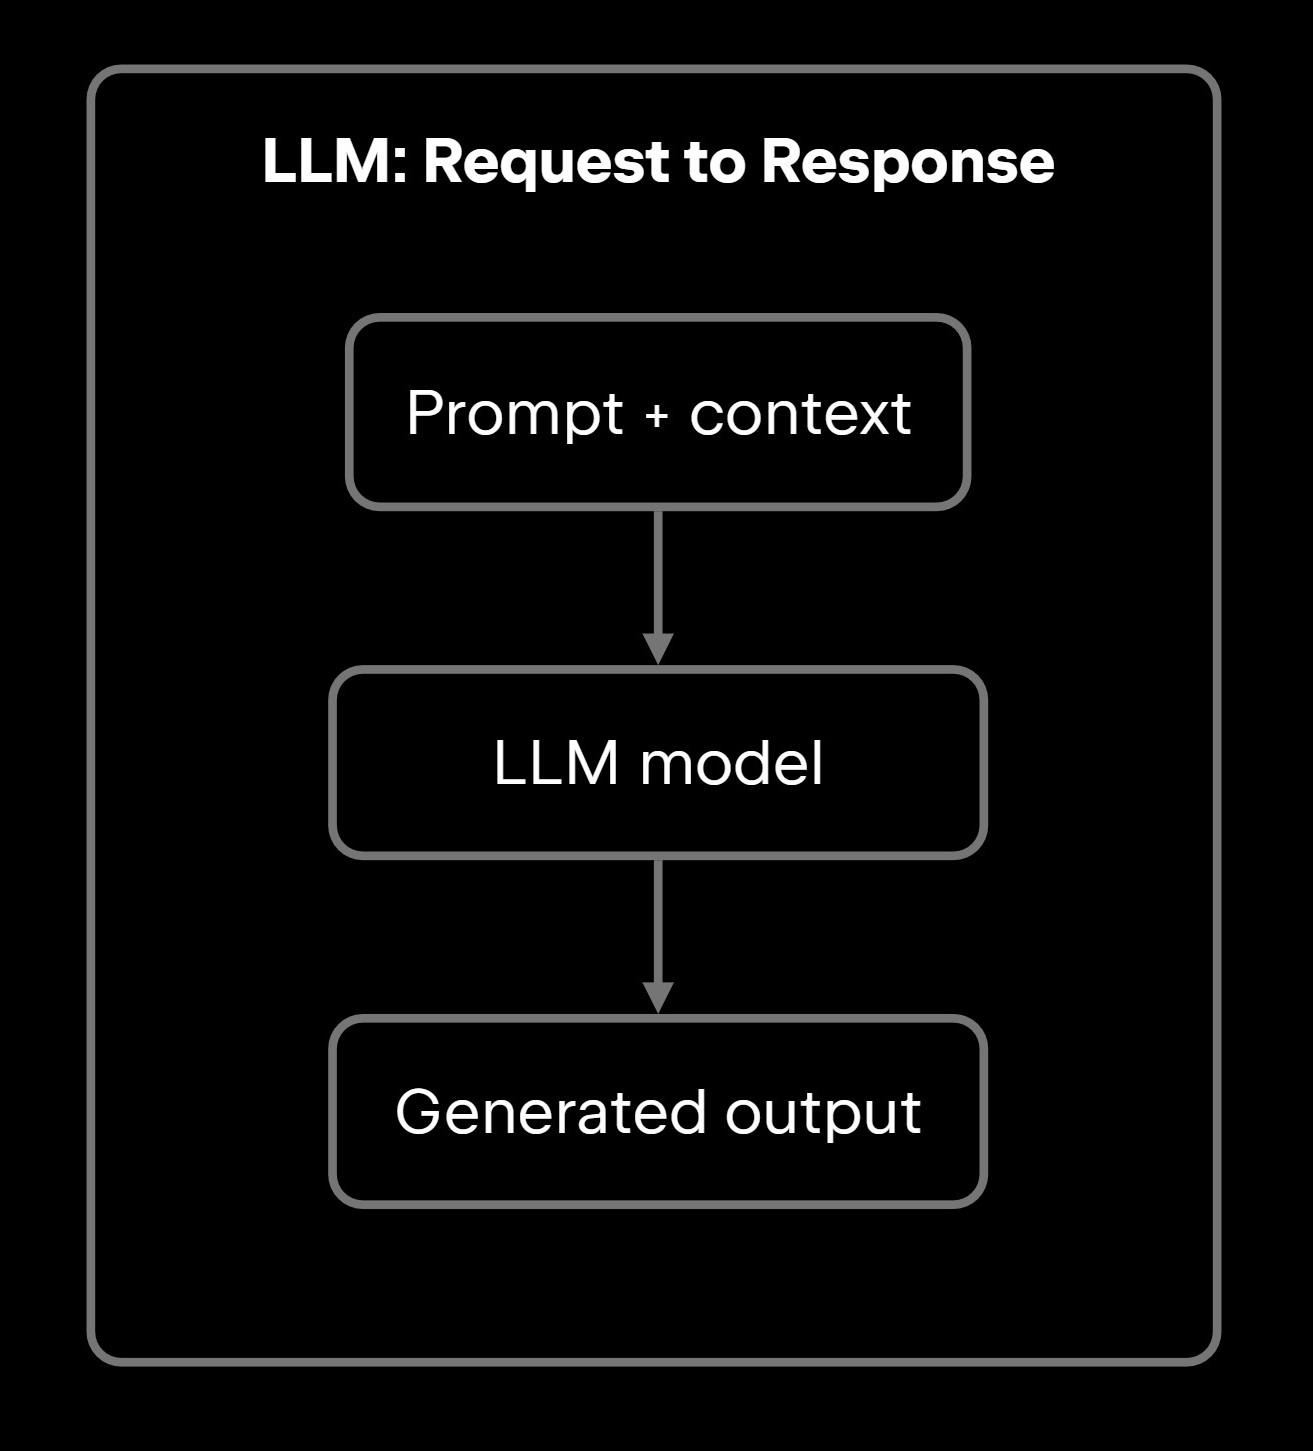
\includegraphics[width=0.48\textwidth]{figures/image2.jpeg}
    \caption{The Monolithic LLM Request-to-Response Paradigm: A stateless, single-turn inference cycle lacking environment feedback and self-correction.}
    \label{fig:llm_req_resp}
\end{figure}

To bridge the gap between static text predictors and goal-directed intelligent actors, the AI research community has advanced toward \textit{Autonomous Agents} \cite{xi2023rise, yao2023react}. An agent is formally defined as an autonomous entity that perceives its environment through sensory observations, maintains internal state and goals, executes deliberate reasoning and planning, and acts upon the environment via tools or actuators \cite{schick2024toolformer}. When an LLM serves as the central cognitive engine (``the brain'') of this construct, it transforms from a passive chat interface into an active problem solver.

\section{The Limits of a Single Agent and the Need for Teams}
While equipping a single LLM with tools, working memory, and prompt chains yields considerable utility, a solo agent rapidly encounters fundamental operational ceilings when confronted with intricate, open-ended real-world challenges:
\begin{enumerate}
    \item \textbf{Outdated and Static Knowledge:} LLM parametric memory is bounded by its training cutoff date. While retrieval mechanisms mitigate this, a single agent often struggles to dynamically arbitrate between conflicting, newly retrieved data points and pre-trained biases.
    \item \textbf{Hallucination and Factuality Decay:} Without external grounding or independent validation, an LLM can generate persuasive yet factually catastrophic outputs. In a solo agent loop, errors made in early steps persist and compound through subsequent planning stages.
    \item \textbf{Brittle Long-Horizon Planning:} Complex tasks require exploring broad solution spaces, decomposing problems into interdependent sub-goals, and backtracking upon failure. Single models exploring deep decision trees frequently suffer from goal drift, hallucinated prerequisites, and contextual distractions.
    \item \textbf{Context Window Exhaustion and Attention Dilution:} As reasoning trajectories expand, packing extensive scratchpads, API schemas, and historical logs into a single context window exhausts token budgets and degrades attention focus (the ``lost-in-the-middle'' phenomenon).
    \item \textbf{Absence of Verification and Cognitive Diversity:} In human organizations, mission-critical operations are never entrusted to a single individual working in total isolation. Instead, multidisciplinary teams distribute labor, challenge assumptions, and audit results. A solitary LLM agent suffers from the absence of peer review: it cannot cross-check its own blind spots.
\end{enumerate}

To transcend these bottlenecks, researchers have established the paradigm of \textbf{LLM-based Multi-Agent Systems (MAS)} \cite{li2024survey, guo2024large}. In an MAS, multiple specialized agents collaborate, negotiate, compete, and communicate. By decomposing monolithic responsibilities into discrete agent profiles (e.g., planners, searchers, coders, critics), multi-agent systems leverage division of labor, modular cognitive architectures, and decentralized verification to solve problems intractable for any single model.

\section{Seminar Objectives}
The core objectives of this technical seminar and report are as follows:
\begin{itemize}
    \item \textbf{Systematic Overview:} Provide a rigorous theoretical overview of LLM-based multi-agent systems, synthesized from authoritative survey literature including Li et al. \cite{li2024survey} and Guo et al. \cite{guo2024large}.
    \item \textbf{Architectural Deconstruction:} Dissect the transition from single-agent cognitive components to the multi-agent interaction layer, detailing profiling, perception, memory architectures, reasoning mechanisms, and interaction topologies.
    \item \textbf{Practical Engineering Case Study:} Present the design, implementation, and empirical evaluation of an autonomous, multi-agent research assistant pipeline developed in Python using LangChain and Groq API.
    \item \textbf{Taxonomy of Applications and Frontiers:} Analyze broad application domains (software development, world simulation, scientific discovery) while systematically outlining open technical challenges, alignment risks, and future research vectors.
\end{itemize}

\section{Organization of the Report}
The remainder of this report is organized as follows:
\begin{itemize}
    \item \textbf{Chapter~\ref{chap:literature_review}} reviews foundational and contemporary literature, presenting a comparative analysis between the two seminal surveys by Li et al. \cite{li2024survey} and Guo et al. \cite{guo2024large}.
    \item \textbf{Chapter~\ref{chap:theoretical_framework}} elaborates the complete theoretical framework: single-agent internals, the five-module multi-agent workflow, memory and knowledge grounding, interaction topologies, and evolution schemes.
    \item \textbf{Chapter~\ref{chap:case_study}} details the practical implementation of our Autonomous Multi-Agent Research Assistant case study, covering system specifications, tool integrations, and experimental critique evaluations.
    \item \textbf{Chapter~\ref{chap:applications}} surveys real-world applications across problem-solving and social simulation spheres.
    \item \textbf{Chapter~\ref{chap:challenges}} investigates prevailing challenges, intrinsic constraints, security considerations, and future frontiers.
    \item \textbf{Chapter~\ref{chap:conclusion}} concludes the report with key takeaways.
\end{itemize}


% ==============================================================================
% CHAPTER 2: LITERATURE REVIEW AND COMPARATIVE SURVEY
% ==============================================================================
\chapter{Literature Review and Comparative Survey}
\label{chap:literature_review}

\section{Evolution of Multi-Agent Systems in Artificial Intelligence}
The investigation of Multi-Agent Systems has deep roots in classical distributed artificial intelligence (DAI). Historically, multi-agent architectures relied on rule-based expert engines, explicit game-theoretic payoffs, or multi-agent reinforcement learning (MARL). In classical MARL, agents learn optimal policies via environmental rewards within Markov Decision Process formulations. However, MARL suffers from exponential state-action space explosion, non-stationarity during decentralized training, low sample efficiency, and an inability to transfer learned behaviors across distinct problem formulations.

The emergence of Large Language Models has revitalized multi-agent research by replacing rigid policy matrices and symbolic predicates with rich natural language representations. Natural language serves as a universal medium for inter-agent communication, environmental reasoning, goal definition, and tool manipulation. In early 2023, Park et al. demonstrated \textit{Generative Agents} \cite{park2023generative}, populating a virtual sandbox (Smallville) with 25 autonomous LLM agents that simulated emergent human sociability, memory reflection, and relationship formation. Concurrently, Yao et al. formulated the \textit{ReAct} paradigm \cite{yao2023react}, interleaving dynamic reasoning traces with environmental tool calls. Subsequently, frameworks like ChatDev \cite{qian2023communicative}, MetaGPT \cite{hong2023metagpt}, and AutoGen \cite{wu2023autogen} demonstrated that structuring LLM interactions according to standard organizational workflows drastically enhances software engineering productivity and multi-agent coordination.

\section{In-Depth Review of Primary Survey Literature}
Given the blistering pace of development, several comprehensive surveys have sought to organize the literature. Two premier landmark works form the cornerstone of this seminar:

\subsection{Li et al. (2024): Workflow-Driven Perspective}
Li, Wang, Zeng, Wu, and Yang \cite{li2024survey} present \textit{``A survey on LLM-based multi-agent systems: workflow, infrastructure, and challenges''} published in \textit{Vicinagearth} (Springer). The primary motivation of Li et al. was that prior agent research was highly fragmented, focusing idiosyncratically on prompt engineering or domain-specific tools without an overarching structural workflow. 

Li et al. unify the field by proposing a comprehensive \textbf{5-module workflow lifecycle}:
\begin{enumerate}
    \item \textbf{Profile:} Defining the persona, domain skills, and constraints of each agent.
    \item \textbf{Perception:} Ingesting environmental feedback, inter-agent messages, and multimodal inputs.
    \item \textbf{Self-Action:} Internal operations including hierarchical memory recall, external knowledge grounding, reasoning, and tool execution.
    \item \textbf{Mutual Interaction:} The coordination layer governing message delivery mechanisms, topological structures, and collaboration scenes.
    \item \textbf{Evolution:} Post-trajectory adaptation through fine-tuning, reflection, prompt updates, and reinforcement learning.
\end{enumerate}
Li et al. categorize multi-agent applications into two overarching domains: \textit{Problem Solving} (goal-driven software engineering, robotics, science experiments) and \textit{World Simulation} (gaming, economic trading, societal behavior, epidemic modeling).

\subsection{Guo et al. (2024): Progress, Communication, and Capability Growth}
Guo, Chen, Wang, Chang, Pei, Chawla, Wiest, and Zhang \cite{guo2024large} present \textit{``Large language model based multi-agents: A survey of progress and challenges''} in the \textit{Proceedings of the 33rd International Joint Conference on Artificial Intelligence (IJCAI-24)}. 

Guo et al. structure the multi-agent landscape around four core axes:
\begin{enumerate}
    \item \textbf{Agent-Environment Interface:} How agents perceive structured, unstructured, and interactive dynamic simulation environments.
    \item \textbf{Agent Profiling:} Methodologies for instantiating diverse agent personas via demographic descriptors, psychology-based traits, and automated character generation.
    \item \textbf{Communication Mechanisms:} Analyzing communication paradigms, message formats (natural language, code, symbolic structures), and coordination protocols (centralized, peer-to-peer, blackboard).
    \item \textbf{Capability Growth:} How multi-agent collectives enhance performance over time via in-context learning, verbal reinforcement, multi-agent debate, and memory accumulation.
\end{enumerate}

\section{Comparative Synthesis of Primary Literature}
Table~\ref{tab:lit_comparison} presents a systematic, comparative synthesis of the two primary survey papers, contrasting their conceptual frameworks, structural categorization, focal strengths, and noted limitations.

\begin{table}[htbp]
\centering
\small
\caption{Systematic Comparative Synthesis of Primary Survey Literature}
\label{tab:lit_comparison}
\begin{tabularx}{\textwidth}{p{3.2cm}X X}
\toprule
\textbf{Dimension} & \textbf{Li et al. (2024) \cite{li2024survey}} & \textbf{Guo et al. (2024) \cite{guo2024large}} \\
\midrule
\textbf{Paper Title} & \textit{A survey on LLM-based multi-agent systems: workflow, infrastructure, and challenges} & \textit{Large language model based multi-agents: A survey of progress and challenges} \\
\addlinespace
\textbf{Authors \& Venue} & X. Li, S. Wang, S. Zeng, Y. Wu, Y. Yang (\textit{Vicinagearth}, Springer) & T. Guo, X. Chen, Y. Wang, et al. (\textit{IJCAI-24}) \\
\addlinespace
\textbf{Core Architectural Framework} & 5-Module Workflow: Profile $\rightarrow$ Perception $\rightarrow$ Self-Action $\rightarrow$ Mutual Interaction $\rightarrow$ Evolution & 4-Quadrant Focus: Environment Interface, Profiling, Communication, Capability Growth \\
\addlinespace
\textbf{Structural Taxonomy} & Workflow-centric decomposition; splits applications into Problem Solving vs. World Simulation & Communication-centric decomposition; categorizes environments into virtual, physical, and hybrid \\
\addlinespace
\textbf{Key Strengths} & Clear end-to-end lifecycle engineering; rigorous breakdown of memory systems, reasoning plans, and evolution & Deep exploration of communication protocols, multi-agent debate mechanisms, and benchmark suites \\
\addlinespace
\textbf{Perspective on Challenges} & Emphasizes intrinsic LLM constraints (hallucination cascade, bias), scaling costs, and system dynamicity & Highlights evaluation subjectivity, inter-agent misalignment, error propagation, and benchmark leakage \\
\bottomrule
\end{tabularx}
\end{table}


% ==============================================================================
% CHAPTER 3: THEORETICAL FOUNDATIONS: FROM SINGLE TO MULTI-AGENT
% ==============================================================================
\chapter{Theoretical Foundations: The Single-to-Multi-Agent Paradigm}
\label{chap:theoretical_framework}

\section{Single-Agent Cognitive Architecture}
Before exploring multi-agent dynamics, it is necessary to examine the cognitive anatomy of a single LLM-based autonomous agent. While a naked LLM merely outputs tokens in response to prompts, an autonomous agent couples the LLM core with four foundational peripheral subsystems: \textit{Memory}, \textit{Planning}, \textit{Tools}, and \textit{Action}, as illustrated in Figure~\ref{fig:single_agent_arch}.

\begin{figure}[htbp]
    \centering
    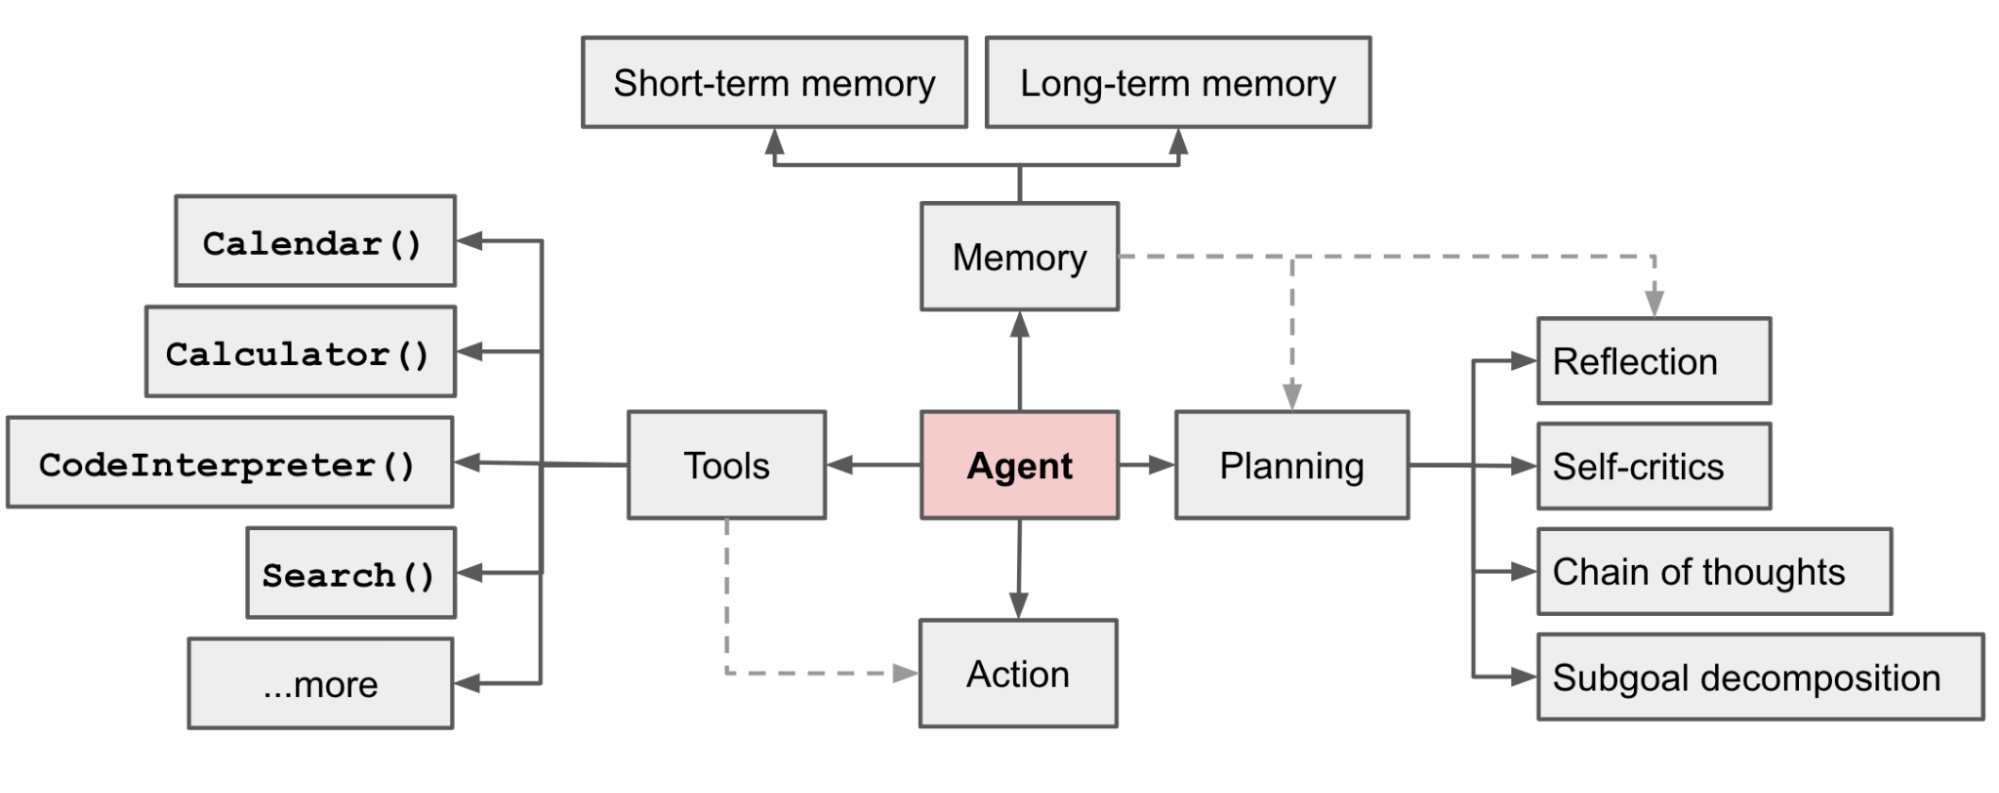
\includegraphics[width=0.88\textwidth]{figures/image3.png}
    \caption{Single-Agent Cognitive Architecture: Integrating the central LLM engine with working memory, tool integration, multi-stage planning, and action dispatch.}
    \label{fig:single_agent_arch}
\end{figure}

\begin{itemize}
    \item \textbf{The Core Agent (Brain):} The foundation model responsible for language comprehension, contextual reasoning, and decision generation.
    \item \textbf{Memory Subsystem:} Divided into short-term working memory (in-context conversational history) and long-term memory (vector databases storing historical episodes and factual embeddings).
    \item \textbf{Planning Subsystem:} Decomposes overarching goals into tractable sub-tasks, performs self-critique, and generates multi-step reasoning traces (Chain-of-Thought, Tree-of-Thoughts) \cite{wei2022chain, yao2024tree}.
    \item \textbf{Tools Subsystem:} External APIs and computational actuators (calculators, web search engines, Python code interpreters, databases) that empower the agent to transcend pure text generation and execute real-world operations \cite{schick2024toolformer}.
    \item \textbf{Action Execution:} The physical or digital dispatch of decisions, executing tool invocations or transmitting textual feedback to the environment.
\end{itemize}

\section{The Unified 5-Module Multi-Agent Framework}
A Multi-Agent System is not simply a collection of disconnected single agents; it is a collective consisting of individual specialized agents coupled with an overarching \textbf{Mutual Interaction Layer}. As formalized by Li et al. \cite{li2024survey} and shown in Figure~\ref{fig:mas_workflow_arch}, each agent maintains its own internal profile, perception, self-action, and evolution loops, while the interaction layer governs message exchanges, collaborative structures, and coordination topologies.

\begin{figure}[htbp]
    \centering
    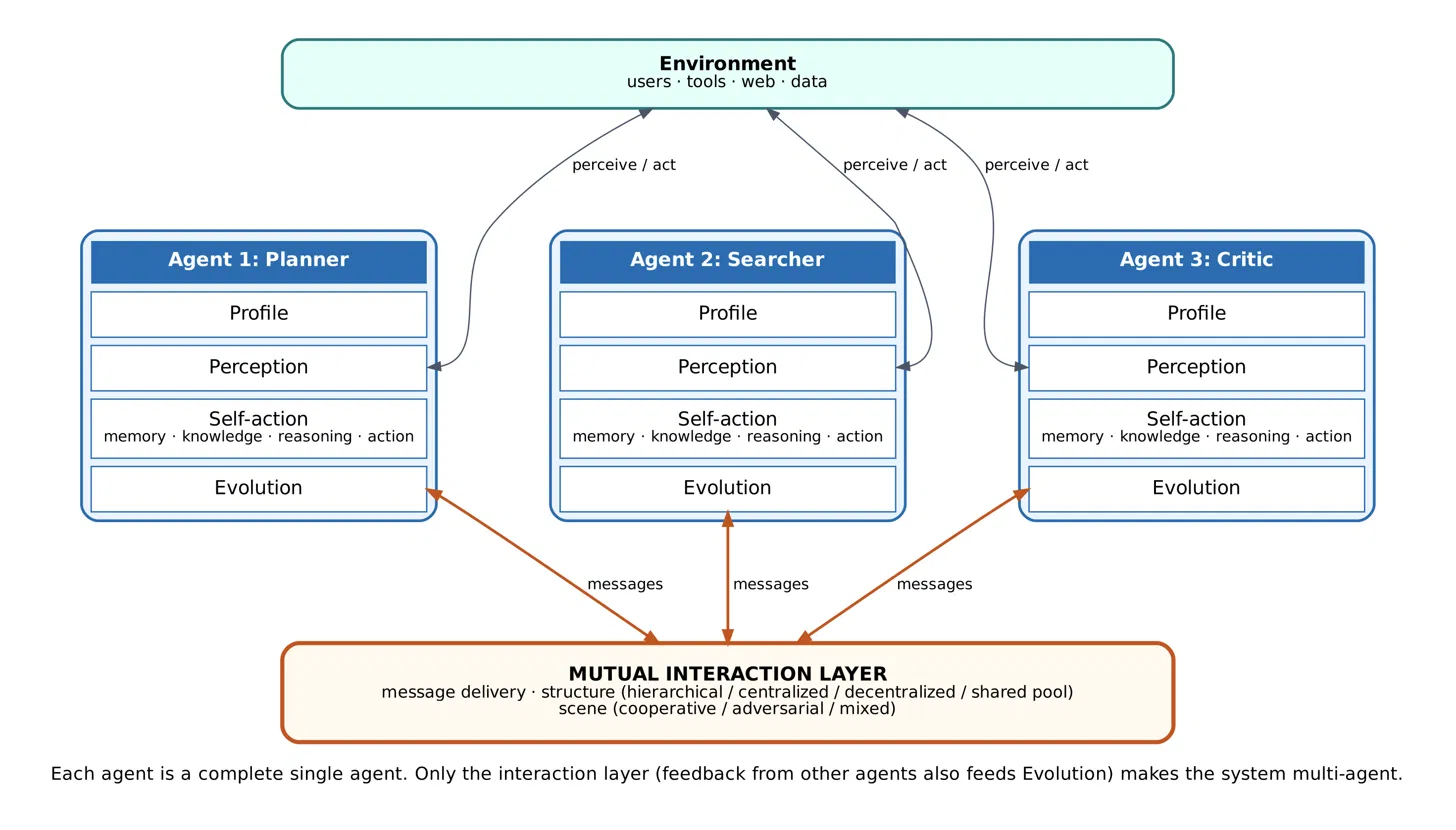
\includegraphics[width=0.92\textwidth]{figures/image4.png}
    \caption{Unified 5-Module Multi-Agent System Framework (Li et al., 2024): Integrating specialized single agents with the Mutual Interaction Layer and Environment.}
    \label{fig:mas_workflow_arch}
\end{figure}

\subsection{Module 1: Agent Profiling}
Agent profiling establishes the identity, behavioral guidelines, domain competencies, and constraints of each participant. Profiling prevents homogeneous behavior, enabling specialized division of labor.
\begin{itemize}
    \item \textbf{Pre-defined Profiling:} The developer manually crafts prompt templates specifying the agent's role, persona, tone, and operational boundaries (e.g., ``You are a senior cybersecurity auditor...'').
    \item \textbf{Contextualized Profiling:} The system dynamically initializes profiles based on incoming task requirements or domain descriptions provided at runtime.
    \item \textbf{Learning-based Profiling:} Agent profiles evolve or are generated automatically through machine learning, fine-tuning, or historical trajectory clustering.
\end{itemize}

\subsection{Module 2: Perception}
Perception denotes an agent's capability to ingest and interpret information from its surrounding context:
\begin{itemize}
    \item \textbf{Perception Sources:} Includes \textit{Environment Messages} (system states, sensor data, web search API results), \textit{Interaction Messages} (direct queries, critiques, or proposals from other agents), and \textit{Self-Reflection Messages} (evaluations of past successes or failures).
    \item \textbf{Modalities:} While predominantly textual, modern multi-agent systems increasingly incorporate visual inputs (screenshots, diagrams) and auditory data, enabling multimodal perception.
\end{itemize}

\subsection{Module 3: Self-Action Mechanisms}
Self-action constitutes the internal computational cycle executed by an agent upon receiving perceptual inputs. This encompasses four critical sub-mechanisms:

\subsubsection{Hierarchical Memory Architectures}
Agents must retain past experiences, facts, and interim decisions without saturating the prompt context window. As depicted in Figure~\ref{fig:memory_arch}, memory is organized into three complementary tiers:
\begin{enumerate}
    \item \textbf{Short-Term Working Memory (STM):} The active conversational context retained within the prompt window.
    \item \textbf{Long-Term Memory (LTM):} Persistent memory decoupled into \textit{Episodic Memory} (specific historical events and task traces), \textit{Semantic Memory} (generalized facts and conceptual knowledge), and \textit{Procedural Memory} (rules, tool syntax, and operational sequences).
    \item \textbf{Memory Storage, Reflection, and Retrieval:} Incoming experiences are stored via addition, merging, or exchange. Through periodic \textit{reflection}, raw episodic trails are synthesized into abstract insights. During task execution, semantic embedding retrieval surfaces the most relevant long-term memory records into current prompts.
\end{enumerate}

\begin{figure}[htbp]
    \centering
    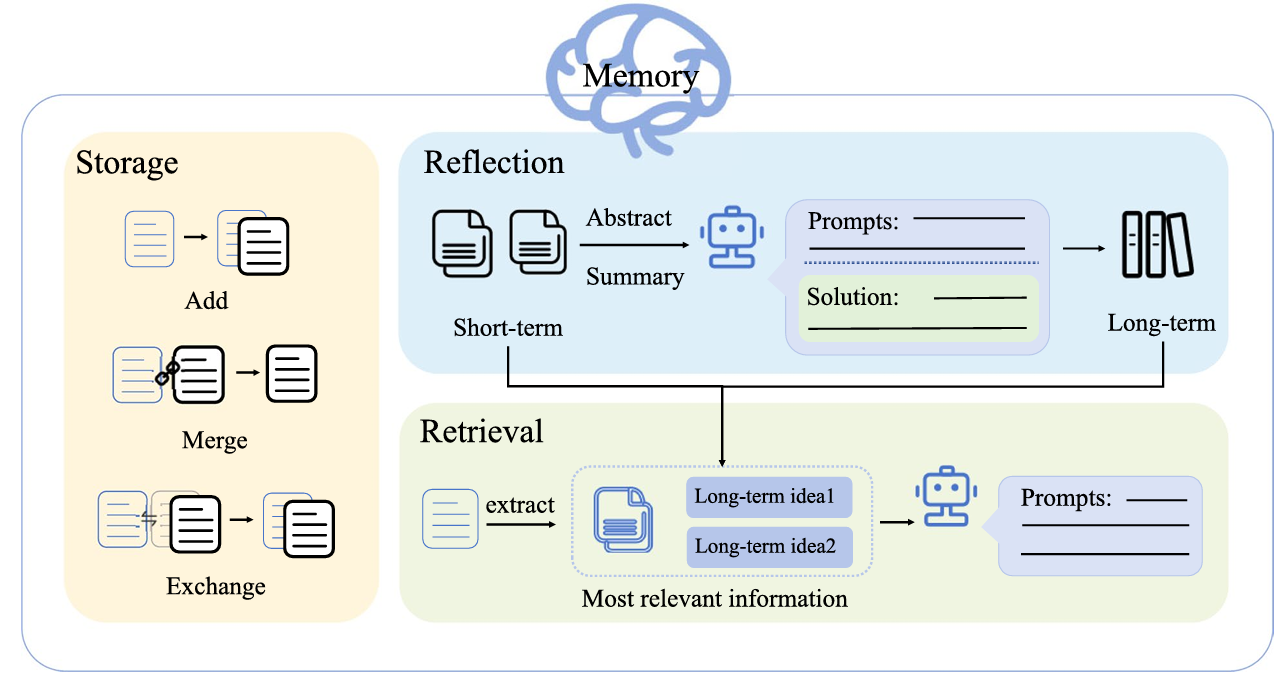
\includegraphics[width=0.88\textwidth]{figures/image5.png}
    \caption{Agent Memory Architecture: Storage operations, reflective summarization, and similarity-based retrieval grounding agent prompts (Li et al., 2024).}
    \label{fig:memory_arch}
\end{figure}

\subsubsection{Knowledge Grounding and Tool Utilization}
LLMs frequently suffer from information lag, hallucinations, and spurious biases. Grounding agents in external knowledge sources is essential for operational reliability, as outlined in Figure~\ref{fig:knowledge_tools}:
\begin{itemize}
    \item \textbf{Structured Queries:} Interfacing with relational databases, knowledge graphs (Wikidata, PubMed), and enterprise registries.
    \item \textbf{Web Scraping and External APIs:} Dynamic execution of live web search (e.g., Tavily API) and HTML scraping (e.g., BeautifulSoup) to harvest real-time data.
    \item \textbf{Retrieval-Augmented Generation (RAG):} Vectorizing external domain corpora to retrieve contextually rich passages, effectively anchoring agent reasoning in verified facts \cite{lewis2020retrieval}.
\end{itemize}

\begin{figure}[htbp]
    \centering
    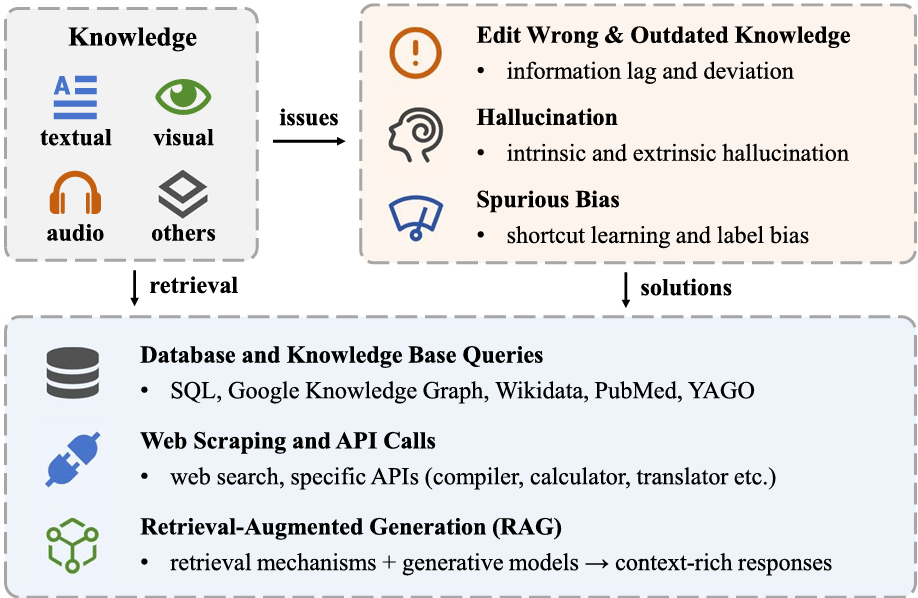
\includegraphics[width=0.85\textwidth]{figures/image6.png}
    \caption{Knowledge Utilization and Tool Grounding: Mitigating outdated knowledge, hallucinations, and biases through database queries, web scraping, and RAG.}
    \label{fig:knowledge_tools}
\end{figure}

\subsubsection{Reasoning and Planning Paradigms}
Generating robust actions requires deliberate planning. As illustrated in Figure~\ref{fig:reasoning_planning}, multi-agent systems contrast two primary planning strategies:
\begin{itemize}
    \item \textbf{One-Step Reasoning and Planning:} The agent ingests the prompt, formulates an immediate, complete sequence of sub-tasks (or multiple candidate trajectories), and executes them sequentially.
    \item \textbf{Multi-Step Reasoning and Planning:} The agent operates iteratively via closed-loop feedback. It generates an immediate sub-plan, evaluates execution results, and dynamically updates subsequent sub-goals based on environmental outcomes.
\end{itemize}

\begin{figure}[htbp]
    \centering
    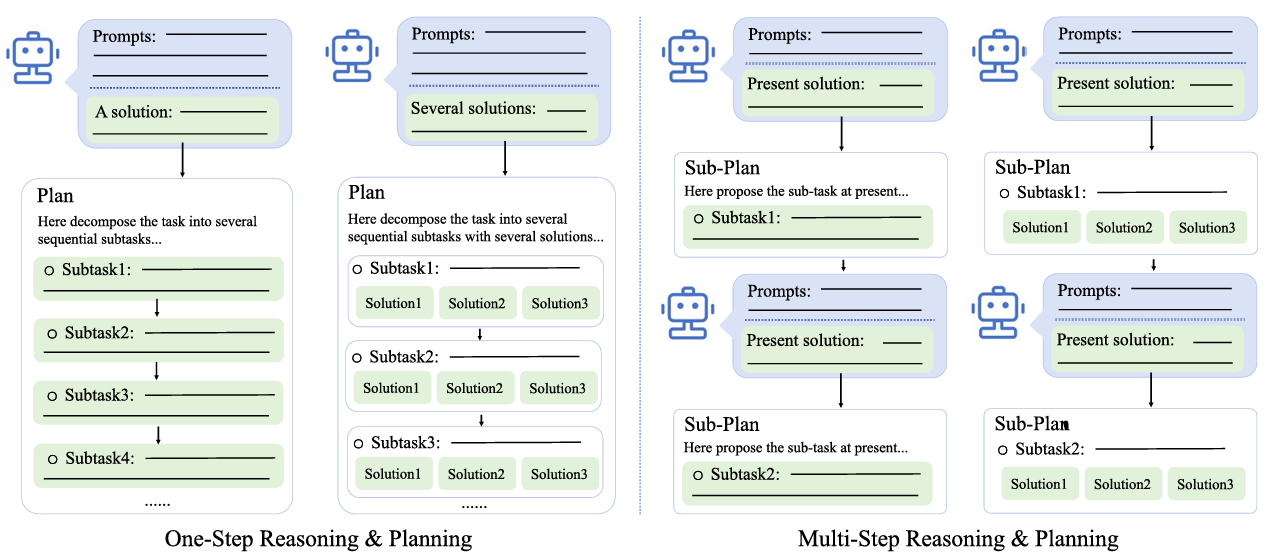
\includegraphics[width=0.92\textwidth]{figures/image7.png}
    \caption{Reasoning and Planning Paradigms: One-Step decomposition versus iterative Multi-Step closed-loop planning (Li et al., 2024).}
    \label{fig:reasoning_planning}
\end{figure}

\subsection{Module 4: Mutual Interaction Layer}
The mutual interaction layer defines the social fabric of the multi-agent system: how agents communicate, coordinate, and organize their collective efforts.

\subsubsection{Message Delivery and Communication Topologies}
Communication protocols fall into distinct structural topologies:
\begin{itemize}
    \item \textbf{Hierarchical Structure:} A leader or manager agent directs tasks to subordinate specialized workers, aggregates their outputs, and enforces quality control.
    \item \textbf{Centralized Structure:} A central coordinator orchestrates all inter-agent traffic in an explicit workflow pipeline.
    \item \textbf{Decentralized (Peer-to-Peer) Structure:} Fully autonomous agents communicate directly without centralized oversight, negotiating or debating solutions collaboratively.
    \item \textbf{Shared Message Pool (Blackboard):} Agents publish updates to and consume messages from a global shared message repository.
\end{itemize}

\subsubsection{Interaction Scenes: Cooperative, Adversarial, and Mixed}
As shown in Figure~\ref{fig:interaction_scenes}, multi-agent collaboration unfolds across three primary interactive scenes:
\begin{enumerate}
    \item \textbf{Cooperative Scenes:} Agents share a unified objective. Coordination can be \textit{Ordered} (a deterministic pipeline where agent $A \rightarrow B \rightarrow C$) or \textit{Unordered} (dynamic collaborative deliberation).
    \item \textbf{Adversarial Scenes:} Agents possess competing objectives or act as debaters. Competitive debate incentivizes agents to scrutinize opposing arguments, effectively filtering out hallucinations.
    \item \textbf{Mixed Scenes:} Blends cooperation and competition. Examples include \textit{Parallel} teams competing against one another while collaborating internally, or \textit{Hierarchical} organizations with internal audit checks.
\end{enumerate}

\begin{figure}[htbp]
    \centering
    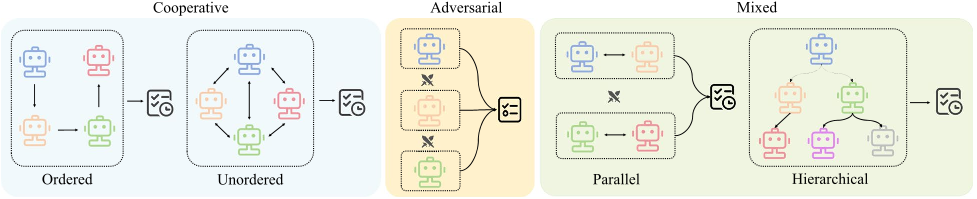
\includegraphics[width=0.92\textwidth]{figures/image8.png}
    \caption{Multi-Agent Interaction Scenes: Cooperative (ordered and unordered), Adversarial debate, and Mixed (parallel and hierarchical) topologies.}
    \label{fig:interaction_scenes}
\end{figure}

\subsection{Module 5: Evolution Mechanisms}
Unlike static pipelines, advanced multi-agent systems exhibit capacity growth over time:
\begin{itemize}
    \item \textbf{Evolution Sources:} Derived from environmental rewards, peer-agent critique feedback, or human-in-the-loop corrections.
    \item \textbf{Evolution Methods:} Encompasses parameter fine-tuning (LoRA, full weights), verbal reinforcement learning (Reflexion \cite{shinn2024reflexion}), prompt self-optimization, and memory accumulation.
    \item \textbf{Dynamic Adjustment:} Agents dynamically refine their system prompts, update procedural guidelines, and purge obsolete records from episodic memory based on post-task critiques.
\end{itemize}


% ==============================================================================
% CHAPTER 4: IMPLEMENTATION CASE STUDY: AUTONOMOUS RESEARCH ASSISTANT
% ==============================================================================
\chapter{Implementation Case Study: Autonomous Research Assistant}
\label{chap:case_study}

\section{System Overview and Architecture}
To substantiate the theoretical foundations of multi-agent workflows, this seminar incorporates a practical engineering implementation: an \textbf{Autonomous Multi-Agent Research Assistant} developed within this project. The system automates the laborious end-to-end workflow of academic research: taking an arbitrary, complex research topic and producing a thoroughly investigated, scraped, synthesized, and rigorously peer-reviewed report with formal citations.

The system is architected as an ordered cooperative pipeline comprising four specialized personas: two autonomous tool-using agents (\textbf{Search Agent} and \textbf{Reader Agent}) and two structured processing chains (\textbf{Writer Chain} and \textbf{Critic Chain}). Figure~\ref{fig:case_study_arch} depicts the complete operational pipeline.

\begin{figure}[htbp]
    \centering
    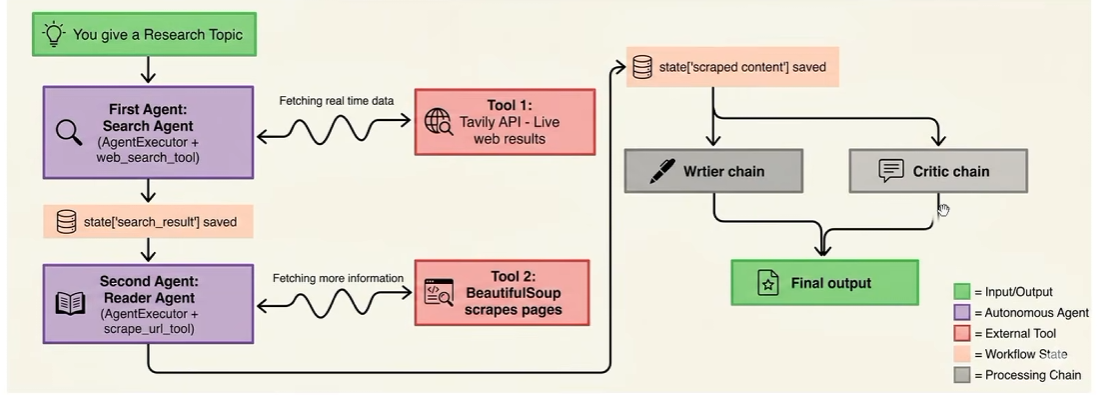
\includegraphics[width=0.95\textwidth]{figures/image9.png}
    \caption{End-to-End Workflow Architecture of the Autonomous Research Assistant: Search Agent, Reader Agent, Writer Chain, and Critic Chain with shared state management.}
    \label{fig:case_study_arch}
\end{figure}

\section{System Specifications and Technology Stack}
The system implementation adheres to modern agentic software engineering principles, leveraging the specifications detailed in Table~\ref{tab:system_specs}.

\begin{table}[htbp]
\centering
\small
\caption{System Implementation Specifications and Technology Stack}
\label{tab:system_specs}
\begin{tabularx}{\textwidth}{p{3.8cm}X}
\toprule
\textbf{Component} & \textbf{Specification / Technology} \\
\midrule
\textbf{Programming Language} & Python 3.10+ \\
\textbf{Agent Framework} & LangChain Core \& LangGraph AgentExecutor \\
\textbf{Inference Engine} & Groq Cloud API (High-throughput LPUs) \\
\textbf{Foundation LLM} & LLaMA-3-70B-Versatile / LLaMA-3.1-8B-Instant (Temperature = 0.0) \\
\textbf{Search Engine Tool} & Tavily Search API (optimized for autonomous AI agents) \\
\textbf{Scraper Tool} & BeautifulSoup4 + HTTP Requests with User-Agent spoofing \\
\textbf{User Interface} & Streamlit (Reactive Dark Theme, interactive telemetry logs) \\
\textbf{State Management} & Centralized Python Dictionary State (\texttt{dict}) \\
\bottomrule
\end{tabularx}
\end{table}

\section{Detailed Agent Roles and Module Implementation}

\subsection{Search Agent (Web Discovery)}
The Search Agent is an autonomous agent instantiated via LangChain's \texttt{create\_agent}. It is equipped with the \texttt{web\_search} tool backed by the Tavily API:
\begin{itemize}
    \item \textbf{Profile / System Prompt:} \textit{``You are a helpful assistant that can search the web and scrape content from URLs.''}
    \item \textbf{Perception:} Ingests the initial research topic provided by the user.
    \item \textbf{Self-Action:} Formulates optimized search queries, queries the Tavily API, and extracts verified titles, URLs, and contextual snippets.
    \item \textbf{Output State:} Writes structured search results into \texttt{state['search\_results']}.
\end{itemize}

\subsection{Reader Agent (Deep Scraping and Extraction)}
The Reader Agent acts as an analytical document consumer. Given the search results, it prioritizes authoritative URLs and executes content extraction:
\begin{itemize}
    \item \textbf{Profile / System Prompt:} \textit{``You are a web-page reader. The user will provide search results containing URLs. Select the most relevant URLs, then call scrape\_url once per URL. The scrape\_url tool accepts exactly one argument named 'url', whose value must be the complete URL string. Never call scrape\_url with query, topn, source, or any other arguments. After scraping, summarize the returned page content.''}
    \item \textbf{Tool Execution:} Invokes \texttt{scrape\_url}, which downloads raw HTML, strips script/style tags via BeautifulSoup, and extracts clean paragraph text.
    \item \textbf{Self-Action:} Condenses noisy web pages into concise, information-dense summaries.
    \item \textbf{Output State:} Writes scraped summaries into \texttt{state['scraped\_content']}.
\end{itemize}

\subsection{Writer Chain (Evidence Synthesis)}
Rather than executing arbitrary tool loops, synthesis is handled by a specialized LLM chain (\texttt{writer\_chain}) with an expanded token context ($\text{max\_tokens} = 2000$):
\begin{itemize}
    \item \textbf{System Prompt:} Directs the model as an expert scientific research writer.
    \item \textbf{Input State:} Concatenates both \texttt{state['search\_results']} and \texttt{state['scraped\_content']}.
    \item \textbf{Strict Mandated Structure:} Compels the model to write a formal 7-section report:
    \begin{enumerate}
        \item Introduction (Significance and scope)
        \item Background (Contextual foundation)
        \item Methodology (Data gathering and retrieval approaches)
        \item Findings (Extracted empirical evidence)
        \item Discussion (Interpretation and implications)
        \item Conclusion (Key takeaways)
        \item References (APA formatted source citations)
    \end{enumerate}
    \item \textbf{Output State:} Writes the final report into \texttt{state['report']}.
\end{itemize}

\subsection{Critic Chain (Peer Review and Evaluation Gate)}
To enforce rigorous quality assurance, the output of the Writer Chain is submitted to an independent \texttt{critic\_chain}:
\begin{itemize}
    \item \textbf{Profile / System Prompt:} \textit{``You are a critical reviewer of research reports. Your task is to evaluate the quality, coherence, and accuracy of the report provided to you.''}
    \item \textbf{Rubric-Based Evaluation:} The Critic scores the report out of 10, enumerates bulleted strengths, specifies actionable areas for improvement, and issues a formal quality verdict: \textbf{Acceptable}, \textbf{Needs Improvement}, or \textbf{Unacceptable}.
    \item \textbf{Output State:} Writes structured evaluation feedback into \texttt{state['feedback']}.
\end{itemize}

\section{State Flow and Execution Traces}
The entire orchestration is managed through a lightweight centralized coordinator (\texttt{run\_multi\_agent\_research\_system}), tracing data across intermediate boundaries:
\begin{equation}
\text{Topic} \xrightarrow{} \texttt{state['search\_results']} \xrightarrow{} \texttt{state['scraped\_content']} \xrightarrow{} \texttt{state['report']} \xrightarrow{} \texttt{state['feedback']}
\end{equation}

In an empirical benchmark evaluating the topic \textit{``LLM based multi-agent systems''}, the pipeline successfully retrieved top contemporary surveys, scraped technical documentation, generated an exhaustive 1,500-word synthesis, and received an 8.5/10 review from the Critic Chain, highlighting high source grounding and clear section organization.


% ==============================================================================
% CHAPTER 5: REAL-WORLD APPLICATIONS OF LLM-MAS
% ==============================================================================
\chapter{Real-World Applications of LLM-MAS}
\label{chap:applications}

As outlined in both primary surveys \cite{li2024survey, guo2024large}, LLM-based multi-agent systems are driving paradigm shifts across two broad application categories: \textit{Problem Solving} and \textit{World Simulation}.

\section{Problem-Solving Domains}

\subsection{Autonomous Software Engineering}
Software development is naturally suited for multi-agent collaboration due to its rigorous, modular lifecycle:
\begin{itemize}
    \item \textbf{ChatDev \cite{qian2023communicative}:} Emulates a virtual software company adhering to the classical waterfall model. Specialized agents take on roles including CEO, CPO, CTO, Programmer, and Reviewer. Through structured communicative dialogues (chat chains), agents collaboratively draft software specifications, code repositories, run unit tests, and resolve compilation errors without human intervention.
    \item \textbf{MetaGPT \cite{hong2023metagpt}:} Encodes Standardized Operating Procedures (SOPs) into multi-agent workflows. MetaGPT mandates that agents communicate via formal Software Development Life Cycle (SDLC) artifacts---including PRDs, system architecture diagrams, and API specifications---mitigating hallucination cascades and reducing communication noise by $80\%$.
\end{itemize}

\subsection{Embodied AI and Robotics}
In physical and virtual environments, multi-agent systems coordinate robotic swarms and gaming avatars:
\begin{itemize}
    \item \textbf{Voyager \cite{wang2023voyager}:} An open-ended lifelong learning agent in Minecraft that combines an automated curriculum planner, an iterative code generation loop for skill acquisition, and a vector-indexed skill library, discovering new items and mastering terrains autonomously.
    \item \textbf{Robotic Swarm Coordination:} Decentralized multi-agent teams decompose warehouse logistics, disaster search-and-rescue, and drone formation flight through high-level LLM task allocation.
\end{itemize}

\subsection{Scientific Discovery and Synthesis}
Multi-agent teams are accelerating scientific discovery by performing autonomous literature exploration, hypothesis generation, and chemical reaction planning (e.g., ChemCrow), verifying reaction safety constraints through specialized critic agents before executing physical lab synthesis.

\section{World Simulation Domains}

\subsection{Societal and Behavioral Simulation}
By assigning diverse demographic and psychographic profiles to agents, researchers simulate complex sociological phenomena:
\begin{itemize}
    \item \textbf{Generative Simulacra \cite{park2023generative}:} Park et al. demonstrated that 25 agents interacting in a virtual town spontaneously disseminated information (organizing a Valentine's Day party), formed social alliances, and scheduled daily activities.
    \item \textbf{Public Opinion and Information Spread:} Simulating rumor propagation, political polarization, and social network consensus dynamics under varying media interventions.
\end{itemize}

\subsection{Financial Trading and Economic Markets}
Multi-agent simulation provides a sandbox for macroeconomic experimentation. Agents modeling distinct risk profiles (momentum traders, value investors, central bankers) interact in simulated equity markets, allowing researchers to study flash crashes, liquidity crises, and the emergent effects of regulatory interest rate shifts.

\subsection{Epidemic and Disease Propagation}
Simulating pathogen transmission across synthetic urban populations, where autonomous agents dynamically alter their mobility and adherence to quarantine measures based on perceived health risks and public announcements.


% ==============================================================================
% CHAPTER 6: CHALLENGES, OPEN PROBLEMS, AND FUTURE DIRECTIONS
% ==============================================================================
\chapter{Challenges, Open Problems, and Future Directions}
\label{chap:challenges}

Despite their remarkable capabilities, LLM-based multi-agent systems face critical architectural, cognitive, and societal challenges that currently impede widespread enterprise deployment.

\section{Intrinsic LLM Constraints}
Multi-agent systems inherit the core frailties of the underlying foundation models:
\begin{enumerate}
    \item \textbf{Black-Box Nature and Interpretability Deficits:} Due to billions of neural weights, explaining the exact causal mechanisms behind an agent's tactical choice remains challenging. In multi-agent settings, this opacity multiplies exponentially across inter-agent conversational exchanges.
    \item \textbf{Hallucination Cascade and Error Propagation:} If an upstream agent introduces a fabricated factual claim or erroneous code snippet, downstream agents operating in good faith frequently treat the input as ground truth. This causes hallucinations to cascade and amplify across the collective.
    \item \textbf{Spurious Bias Amplification:} Cultural, demographic, or algorithmic biases present in training data can become mutually reinforced during collaborative peer interactions, leading to unaligned group consensus.
\end{enumerate}

\section{Scalability and Coordination Bottlenecks}
Scaling multi-agent systems from a handful of agents to hundreds or thousands introduces severe infrastructural bottlenecks:
\begin{itemize}
    \item \textbf{Token Consumption and Financial Cost:} Extensive inter-agent chat logs consume massive token volumes, resulting in substantial financial API expenses and high inference latency.
    \item \textbf{Communication Noise and Dialogue Loops:} In unconstrained peer-to-peer topologies, agents can enter endless conversational loops or introduce conversational drift, diluting the primary mission objective.
\end{itemize}

\section{Security, Safety, and Misuse Vulnerabilities}
Multi-agent collaboration introduces novel threat vectors:
\begin{itemize}
    \item \textbf{Adversarial Injection and Jailbreak Cascades:} An attacker can inject a malicious prompt into an external data source (e.g., a scraped website). When the Search Agent ingests this poisoned snippet, it can propagate prompt injection attacks to downstream planner and execution agents.
    \item \textbf{Autonomous Cyber-Attacks and Misuse:} Malicious actors can deploy decentralized multi-agent swarms to conduct autonomous vulnerability scanning, phishing campaign orchestration, and disinformation generation.
\end{itemize}

\section{Future Research Horizons}
To overcome these obstacles, several promising research frontiers are actively developing:
\begin{itemize}
    \item \textbf{Artificial Collective Intelligence:} Developing principled communication compression protocols, semantic consensus algorithms, and game-theoretic voting mechanisms to maximize group problem-solving while minimizing token overhead.
    \item \textbf{Agent-as-a-Service (AaaS):} Modular cloud hosting architectures enabling organizations to rent specialized, pre-trained agent personas on demand, seamlessly interoperating across cloud boundaries.
    \item \textbf{Standardized Tool Protocols (The Model Context Protocol):} Anthropic's open-source \textit{Model Context Protocol (MCP)} \cite{anthropic2024mcp} represents a vital step forward, establishing a universal, secure, client-host-server protocol for connecting AI agents to local and remote tool ecosystems, eliminating proprietary one-off integrations.
\end{itemize}


% ==============================================================================
% CHAPTER 7: CONCLUSION
% ==============================================================================
\chapter{Conclusion}
\label{chap:conclusion}

The transition from solitary, monolithic Large Language Models to communicative, cooperative Multi-Agent Systems marks a pivotal paradigm shift in artificial intelligence. While single models hit undeniable operational ceilings when tackling long-horizon, mission-critical problems, multi-agent collectives leverage specialization, modular cognitive architectures, tool grounding, and iterative peer review to achieve emergent problem-solving capabilities.

This seminar report has conducted an exhaustive, structured survey of the LLM-MAS landscape:
\begin{itemize}
    \item Synthesizing the foundational survey literature of Li et al. \cite{li2024survey} and Guo et al. \cite{guo2024large}, we formalized the universal \textbf{5-module workflow lifecycle}: Profile, Perception, Self-Action, Mutual Interaction, and Evolution.
    \item We deeply analyzed the internal cognitive mechanisms of agents, including hierarchical memory systems (STM, LTM, episodic, semantic, procedural), knowledge grounding against hallucinations via RAG and web scraping, and multi-step reasoning plans.
    \item We explored inter-agent coordination across hierarchical, centralized, and peer-to-peer topologies within cooperative, adversarial, and mixed interaction scenes.
    \item We bridged theoretical paradigms with software engineering by demonstrating an end-to-end \textbf{Autonomous Multi-Agent Research Assistant} pipeline that automates web search, scraping, synthesis, and critique.
    \item Finally, we mapped out real-world application domains across software development, robotics, and social simulation, while addressing core challenges in hallucination cascades, communication scalability, and alignment.
\end{itemize}

As standardized protocols such as MCP mature and collective intelligence algorithms evolve, multi-agent systems will serve as the indispensable architectural bedrock for the next generation of robust, trustworthy, and autonomous AI systems.


% ==============================================================================
% BIBLIOGRAPHY
% ==============================================================================
\newpage
\addcontentsline{toc}{chapter}{References}
\bibliographystyle{ieeetr}
\bibliography{references}

\end{document}
